\chapter{Methodology}
About one to two pages.
Describe the way you went about your project:
\begin{itemize}
\item Agile / incremental and iterative approach to development. Planning, meetings.
\item What about validation and testing? Junit or some other framework.
\item If team based, did you use GitHub during the development process.
\item Selection criteria for algorithms, languages, platforms and technolo-gies.
\end{itemize}
Check out the nice graphs in Figure \ref{tikz:graphs}, and the nice diagram in Figure \ref{tikz:mydiagram}.
\begin{figure}
	\centering
	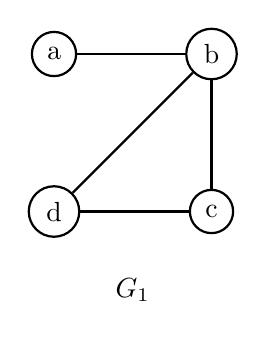
\begin{tikzpicture}
	\begin{scope}[every node/.style={circle,thick,draw}]
	\node (a) at (0,2) {a};
	\node (b) at (2,2) {b};
	\node (c) at (2,0) {c};
	\node (d) at (0,0) {d};
	\end{scope}
	\begin{scope}[every edge/.style={draw=black,thick}]
	\path (a) edge (b);
	\path (b) edge (c);
	\path (b) edge (d);
	\path (c) edge (d);
	\end{scope}
	\node () at (1,-1) {$G_1$};
	\end{tikzpicture}
	\hspace{1.5cm}
	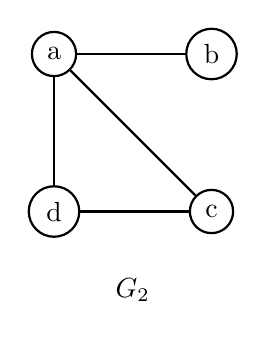
\begin{tikzpicture}
	\begin{scope}[every node/.style={circle,thick,draw}]
	\node (1) at (0,2) {a};
	\node (2) at (2,2) {b};
	\node (3) at (2,0) {c};
	\node (4) at (0,0) {d};
	\end{scope}
	\begin{scope}[every edge/.style={draw=black,thick}]
	\path (1) edge (2);
	\path (1) edge (3);
	\path (1) edge (4);
	\path (3) edge (4);
	\end{scope}
	\node () at (1,-1) {$G_2$};
	\end{tikzpicture}
	\caption{Nice pictures}
	\label{tikz:graphs}
\end{figure}


\begin{figure}
	\centering
	\begin{tikzpicture}[node distance=6cm]
	\node (a) [rect] {A Big Blue Block};
	\node (b) [oval, right of=a] {And His Oval Friend};
	\draw [line] (a) -- (b);
	\end{tikzpicture}
	\caption{Nice pictures}
	\label{tikz:graphs}
\end{figure}